\documentclass[11pt]{article}

\usepackage[margin=1in]{geometry}
\usepackage{amsmath,amssymb,mathtools,bm}
\usepackage{microtype}
\usepackage{amsthm}
\usepackage{booktabs}
\usepackage{array}
\usepackage{graphicx}
\usepackage[numbers,sort&compress]{natbib}
\graphicspath{{figures/}}
\usepackage[colorlinks=true,linkcolor=blue,citecolor=blue,urlcolor=blue]{hyperref}

\theoremstyle{plain}
\newtheorem{proposition}{Proposition}[section]
\newtheorem{assumption}[proposition]{Assumption}
\newtheorem{lemma}[proposition]{Lemma}
\newtheorem{remark}[proposition]{Remark}

\newcommand{\rr}{\bm r}
\newcommand{\kk}{\bm k}
\newcommand{\PP}{P}
\newcommand{\Id}{I}
\newcommand{\erfc}{\operatorname{erfc}}
\newcommand{\erf}{\operatorname{erf}}
\newcommand{\cT}{\mathcal{T}}
\newcommand{\Range}{\operatorname{Range}}
% Allow line breaks after underscores in file and script names.
\DeclareRobustCommand{\_}{\textunderscore\allowbreak}

\title{Notebook}
\author{}
\date{}

\begin{document}
\maketitle

\section{Introduction}
\label{sec:intro}

% Introduction: to be written.

\section{Screened longitudinal friction kernel}
\label{sec:kernel}

\subsection{Kernel and Gaussian-scale representation}

We consider the purely longitudinal matrix-valued kernel
\begin{equation}
\label{eq:kernel}
K_\kappa(\rr)
=
\frac{e^{-\kappa r}}{r}\,\PP(\rr),
\qquad
\PP(\rr)=\frac{\rr\rr^{\mathsf T}}{r^2},
\qquad
r=|\rr|,
\qquad
\kappa>0.
\end{equation}
Throughout, \(\kk\) denotes the Fourier wave vector, \(k=|\kk|\ge 0\), and
\(\xi>0\) is the Ewald splitting parameter.

\begin{proposition}[Gaussian-scale representation]
\label{prop:gauss-scale}
The kernel in Eq.~\eqref{eq:kernel} satisfies
\begin{equation}
\label{eq:gauss-scale}
K_\kappa(\rr)
=
\rr\rr^{\mathsf T}
\int_0^\infty
\rho_\kappa(s)e^{-s r^2}\,ds,
\end{equation}
with the nonnegative weight
\begin{equation}
\label{eq:rho}
\rho_\kappa(s)
=
\frac{1}{\sqrt{\pi}}
\int_0^s
t^{-1/2}
e^{-\kappa^2/(4t)}\,dt
=
\frac{2\sqrt{s}}{\sqrt{\pi}}
e^{-\kappa^2/(4s)}
+
\kappa\left[
\erf\!\left(
\frac{\kappa}{2\sqrt{s}}
\right)-1
\right].
\end{equation}
\end{proposition}

The proof is given in Appendix~\ref{app:gauss-scale}.

\subsection{Ewald splitting}

We split the Gaussian scales in Eq.~\eqref{eq:gauss-scale} at \(s=\xi^2\):
\begin{align}
K_\kappa^L(\rr)
&=
\rr\rr^{\mathsf T}
\int_0^{\xi^2}
\rho_\kappa(s)e^{-s r^2}\,ds,
\\
K_\kappa^S(\rr)
&=
\rr\rr^{\mathsf T}
\int_{\xi^2}^{\infty}
\rho_\kappa(s)e^{-s r^2}\,ds,
\end{align}
o that $K_\kappa=K_\kappa^S+K_\kappa^L$. Since
\(\rr\rr^{\mathsf T}=r^2\PP(\rr)\), both pieces remain purely longitudinal,
\begin{equation}
K_\kappa^{S/L}(\rr)
=
\theta_{S/L}(r)\PP(\rr),
\end{equation}
where
\begin{align}
\theta_L(r)
&=
r^2
\int_0^{\xi^2}
\rho_\kappa(s)e^{-s r^2}\,ds,
\\
\theta_S(r)
&=
r^2
\int_{\xi^2}^{\infty}
\rho_\kappa(s)e^{-s r^2}\,ds.
\end{align}
Because \(\rho_\kappa(s)\ge 0\), both $\theta_L(r)\ge0$ and
$\theta_S(r)\ge0$, so each real-space piece is pointwise positive
semidefinite. Closed-form expressions for $\theta_L$ and $\theta_S$ are
given in Appendix~\ref{app:closed-form}.

\subsection{Localization in real and Fourier space}

We use the Fourier convention
\begin{equation}
\widehat f(\kk)
=
\int_{\mathbb R^3}
e^{-i\kk\cdot\rr}f(\rr)\,d\rr.
\end{equation}

\begin{proposition}[Gaussian localization]
\label{prop:localization}
The short-range kernel satisfies
\begin{equation}
\label{eq:KS-asym}
K_\kappa^S(\rr)
\sim
\rho_\kappa(\xi^2)
e^{-\xi^2r^2}
\PP(\rr),
\qquad
r\to\infty.
\end{equation}
The long-range kernel has the Fourier transform
\begin{equation}
\label{eq:KL-fourier}
\widehat K_\kappa^L(\kk)
=
A_{\kappa,\xi}(k)\Id
+
B_{\kappa,\xi}(k)\kk\kk^{\mathsf T},
\end{equation}
where
\begin{align}
A_{\kappa,\xi}(k)
&=
\frac{\pi^{3/2}}{2}
\int_0^{\xi^2}
\rho_\kappa(s)s^{-5/2}
e^{-k^2/(4s)}\,ds,
\\
B_{\kappa,\xi}(k)
&=
-\frac{\pi^{3/2}}{4}
\int_0^{\xi^2}
\rho_\kappa(s)s^{-7/2}
e^{-k^2/(4s)}\,ds,
\end{align}
and $B_{\kappa,\xi}(k)=A'_{\kappa,\xi}(k)/k$ for $k>0$. As $k\to\infty$,
\begin{equation}
\label{eq:lambda-par-asym}
A_{\kappa,\xi}(k)
\sim
\frac{2\pi^{3/2}}{\xi k^2}
\rho_\kappa(\xi^2)
e^{-k^2/(4\xi^2)},
\qquad
A_{\kappa,\xi}(k)
+
k^2B_{\kappa,\xi}(k)
\sim
-
\frac{\pi^{3/2}}{\xi^3}
\rho_\kappa(\xi^2)
e^{-k^2/(4\xi^2)},
\end{equation}
and consequently
\begin{equation}
\label{eq:KL-decay}
\left\|
\widehat K_\kappa^L(\kk)
\right\|_2
\sim
\frac{\pi^{3/2}}{\xi^3}
\rho_\kappa(\xi^2)
e^{-k^2/(4\xi^2)},
\qquad
k\to\infty.
\end{equation}
\end{proposition}

The proof is given in Appendix~\ref{app:localization}. The value of
$\widehat K_\kappa^L$ at \(k=0\) is obtained directly from the integral
formulas.

The truncation errors of the two pieces are measured by the continuum
tail quantities
\begin{equation}
\label{eq:EF}
E_S(r_c)
=
\int_{|\rr|>r_c}
\|K_\kappa^S(\rr)\|_2\,d\rr,
\qquad
E_F(k_c)
=
\frac{1}{(2\pi)^3}
\int_{|\kk|>k_c}
\left\|
\widehat K_\kappa^L(\kk)
\right\|_2\,d\kk.
\end{equation}
By Proposition~\ref{prop:localization} (see Appendix~\ref{app:localization}),
\begin{equation}
\label{eq:tails}
E_S(r_c)
\sim
\frac{2\pi}{\xi^2}
\rho_\kappa(\xi^2)
r_c e^{-\xi^2r_c^2},
\qquad
E_F(k_c)
\sim
\frac{1}{\sqrt{\pi}\,\xi}
\rho_\kappa(\xi^2)
k_c
e^{-k_c^2/(4\xi^2)}.
\end{equation}
The quantity \(E_F\) is only a continuum asymptotic proxy for the
reciprocal tail. A fully discrete periodic PPPM error estimate also depends
on the reciprocal lattice, mesh spacing, assignment order, aliasing, and
interpolation; these effects are analyzed in Section~\ref{sec:pm}.

\subsection{Leading-order balance}

Balancing the dominant exponential rates
$e^{-\xi^2r_c^2}$ and $e^{-k_c^2/(4\xi^2)}$ in Eq.~\eqref{eq:tails} gives
\begin{equation}
\xi r_c
\approx
\frac{k_c}{2\xi},
\qquad\text{or equivalently}\qquad
\xi^2
\approx
\frac{k_c}{2r_c}.
\end{equation}
Increasing \(\xi\) makes the real-space part more localized but broadens
the reciprocal-space contribution, while decreasing \(\xi\) does the
opposite.

\subsection{Pointwise positivity versus Fourier-multiplier signs}

The real-space positivity of the split kernels should not be confused with
positive semidefiniteness of the Fourier multiplier. By
Eq.~\eqref{eq:KL-fourier}, the eigenvalue of $\widehat K_\kappa^L(\kk)$ on
vectors orthogonal to $\kk$ is $\lambda_\perp(k)=A_{\kappa,\xi}(k)$, whereas
the eigenvalue in the $\kk$ direction is
\begin{equation}
\lambda_\parallel(k)
=
A_{\kappa,\xi}(k)+k^2B_{\kappa,\xi}(k)
=
A_{\kappa,\xi}(k)+kA'_{\kappa,\xi}(k).
\end{equation}
By Eq.~\eqref{eq:lambda-par-asym}, $\lambda_\parallel(k)<0$ for large $k$,
so the Fourier multiplier is generally not positive semidefinite. This
does not contradict the pointwise real-space property
$K_\kappa^L(\rr)\succeq0$. Only the latter enters the graph-Laplacian
argument below.

\section{Fast periodic graph-Laplacian action}
\label{sec:pm}

This section concerns the particle graph and its particle--mesh
discretization. We use only two properties established in
Section~\ref{sec:kernel}: the periodic real-space long-range pair kernel
$K_\kappa^{L,\mathrm{per}}$ is pointwise positive semidefinite, and its
Fourier multiplier has the Gaussian decay of Eq.~\eqref{eq:KL-decay}.

\subsection{Finite reciprocal truncation and a spectral-gap criterion}

For a cubic periodic cell of volume $V=L^3$, let
\begin{equation}
\mathcal K
=
\frac{2\pi}{L}\mathbb Z^3.
\end{equation}
The exact periodic long-range kernel is represented by
\begin{equation}
K_\kappa^{L,\mathrm{per}}(\rr)
=
\frac1V
\sum_{\kk\in\mathcal K}
\widehat K_\kappa^L(\kk)e^{i\kk\cdot\rr}.
\end{equation}
After a reciprocal cutoff $k_c$,
\begin{equation}
K_\kappa^{L,k_c}(\rr)
=
\frac1V
\sum_{|\kk|\le k_c}
\widehat K_\kappa^L(\kk)e^{i\kk\cdot\rr}.
\end{equation}
Define the omitted tail
\begin{equation}
R_{k_c}(\rr)
=
K_\kappa^{L,k_c}(\rr)
-
K_\kappa^{L,\mathrm{per}}(\rr).
\end{equation}
Then
\begin{equation}
\|R_{k_c}(\rr)\|_2
\le
\frac1V
\sum_{|\kk|>k_c}
\|\widehat K_\kappa^L(\kk)\|_2.
\end{equation}
If $\Gamma_L^{k_c}$ is formed from the truncated pair response using the
same degree-minus-weight construction, Lemma~\ref{lem:pair-response} in
Appendix~\ref{app:pair-response} gives
\begin{equation}
\label{eq:trunc-bound}
\|\Gamma_L^{k_c}-\Gamma_L\|_2
\le
2\max_i
\sum_{j\ne i}
\|R_{k_c}(q_i-q_j)\|_2.
\end{equation}
A configuration-independent but generally pessimistic consequence is
\begin{equation}
\label{eq:trunc-pessimistic}
\|\Gamma_L^{k_c}-\Gamma_L\|_2
\le
\frac{2(N-1)}{V}
\sum_{|\kk|>k_c}
\|\widehat K_\kappa^L(\kk)\|_2.
\end{equation}
The Gaussian Fourier asymptotics imply the expected fixed-system rate
\begin{equation}
\|\Gamma_L^{k_c}-\Gamma_L\|_2
=
\mathcal{O}\!\left(
k_c e^{-k_c^2/(4\xi^2)}
\right),
\end{equation}
although the worst-case prefactor inherited from
Eq.~\eqref{eq:trunc-pessimistic} can be very conservative.

Let
\begin{equation}
\cT
=
\operatorname{span}
\{\mathbf 1\otimes e_1,
\mathbf 1\otimes e_2,
\mathbf 1\otimes e_3\}.
\end{equation}
Assume for the moment that the exact graph has no null vectors beyond
translations, and define the restricted spectral gap
\begin{equation}
\label{eq:gap}
\lambda_*
=
\min_{\substack{X\perp\cT\\ \|X\|=1}}
X^{\mathsf T}\Gamma_LX
>0.
\end{equation}

\begin{proposition}[PSD preservation under a small reciprocal perturbation]
\label{prop:psd-trunc}
If $\Gamma_L^{k_c}$ preserves the translation nullspace and
\begin{equation}
\|\Gamma_L^{k_c}-\Gamma_L\|_2<\lambda_*,
\end{equation}
then $\Gamma_L^{k_c}\succeq0$.
\end{proposition}

\begin{proof}
For $X\perp\cT$ with $\|X\|=1$,
\begin{align}
X^{\mathsf T}\Gamma_L^{k_c}X
&=
X^{\mathsf T}\Gamma_LX
+
X^{\mathsf T}(\Gamma_L^{k_c}-\Gamma_L)X
\\
&\ge
\lambda_*
-
\|\Gamma_L^{k_c}-\Gamma_L\|_2
>0.
\end{align}
On $\cT$, both operators vanish.
\end{proof}

The condition in Proposition~\ref{prop:psd-trunc} is sufficient but not
necessary. A truncated pair kernel
can fail to be pointwise semidefinite while the corresponding graph
Laplacian remains positive semidefinite.

\subsection{Symmetric particle--mesh discretization}

Let $P_h$ denote spreading from particles to a periodic mesh and let
\begin{equation}
I_h=P_h^{\mathsf T}
\end{equation}
be the adjoint gathering operator with consistent normalization. Let $F_h$
be the discrete Fourier transform and let $G_h(\kk)$ be an even,
real-symmetric tensor influence function. The particle response is
\begin{equation}
W_h
=
I_hF_h^{-1}G_hF_hP_h.
\end{equation}
Adjoint transfer and an even symmetric multiplier imply that $W_h$ is
symmetric. Rather than using $W_h$ directly as a friction matrix, define
\begin{equation}
\label{eq:pm-graph}
(\widetilde\Gamma_h^LX)_i
=
\left(\sum_j(W_h)_{ij}\right)x_i
-
\sum_j(W_h)_{ij}x_j.
\end{equation}
The self response cancels algebraically, so the block-row sums vanish
exactly and the translation modes are preserved for every mesh and particle
configuration. Symmetry and row-zero structure, however, do not by
themselves guarantee positive semidefiniteness.

If $K^h_{ij}$ denotes the complete approximate pair response and
\begin{equation}
E_{ij}=K^h_{ij}-K_{ij},
\end{equation}
define
\begin{equation}
\epsilon_{\mathrm{op}}
=
2\max_i\sum_{j\ne i}\|E_{ij}\|_2.
\end{equation}
Lemma~\ref{lem:pair-response} gives
\begin{equation}
\label{eq:op-bound}
\|\widetilde\Gamma_h-\Gamma\|_2
\le
\epsilon_{\mathrm{op}}.
\end{equation}
Therefore, if the exact graph has restricted gap $\lambda_*$, defined in
Eq.~\eqref{eq:gap}, and
\begin{equation}
\epsilon_{\mathrm{op}}<\lambda_*,
\end{equation}
then the raw particle--mesh graph is already positive semidefinite and no
stabilization is required.

If this sufficient certificate is not available, one may retain the
translation-preserving fallback stabilization
\begin{equation}
\label{eq:stabilized}
\Gamma_h
=
\widetilde\Gamma_h
+
\delta_h\Pi,
\qquad
\Pi
=
\left(I_N-\frac1N\mathbf1\mathbf1^{\mathsf T}\right)\otimes I_3,
\end{equation}
with
\begin{equation}
\delta_h
\ge
\max\left\{
0,-\lambda_{\min}
\left(
\widetilde\Gamma_h|_{\Range\Pi}
\right)
\right\}.
\end{equation}

\begin{proposition}[Stabilized operator]
\label{prop:stabilized}
The operator $\Gamma_h$ is symmetric positive semidefinite, satisfies
$\Gamma_h t=0$ for every $t\in\cT$, and obeys
\begin{equation}
\|\Gamma_h-\Gamma\|_2\le\epsilon_{\mathrm{op}}+\delta_h.
\end{equation}
\end{proposition}

The proof is given in Appendix~\ref{app:pair-response}. The conservative choice $\delta_h=\epsilon_{\mathrm{op}}$ is always
certified; in the tests of Section~\ref{sec:exp-action} the smallest eigenvalue on $\Range\Pi$ moved by at most
$41\%$ of $\|\widetilde\Gamma_h-\Gamma\|_2$.

\subsection{Complete off-grid mesh-response decomposition}

The mesh error is most transparent when the aliases are kept explicitly.
Let
\begin{equation}
\kk_n
=
\kk+\frac{2\pi}{h}n,
\qquad n\in\mathbb Z^3,
\end{equation}
and let $\widehat W_h$ be the Fourier transform of the assignment window.
For a particle at $q$, define the deposited amplitude
\begin{equation}
S_h(\kk,q)
=
\sum_{n\in\mathbb Z^3}
\widehat W_h(\kk_n)e^{-i\kk_n\cdot q}.
\end{equation}
Separate the principal contribution and the aliases:
\begin{align}
S_0(\kk,q)
&=
\widehat W_h(\kk)e^{-i\kk\cdot q},
\\
A_h(\kk,q)
&=
\sum_{n\ne0}
\widehat W_h(\kk_n)e^{-i\kk_n\cdot q}.
\end{align}
Define the relative alias factor
\begin{equation}
\alpha_h(\kk,q)
=
\frac{A_h(\kk,q)}
{\widehat W_h(\kk)e^{-i\kk\cdot q}},
\end{equation}
so that
\begin{equation}
S_h(\kk,q)
=
\widehat W_h(\kk)e^{-i\kk\cdot q}
\left[1+\alpha_h(\kk,q)\right].
\end{equation}
The phase factor
\begin{equation}
e^{-i(2\pi/h)n\cdot q}
\end{equation}
inside $\alpha_h$ shows explicitly that a finite mesh response depends on
particle positions relative to the grid, not only on pair separation.

Define
\begin{equation}
H_h(\kk)
=
|\widehat W_h(\kk)|^2G_h(\kk),
\qquad
D_h(\kk)
=
H_h(\kk)-\widehat K_\kappa^L(\kk).
\end{equation}
A direct computation (Appendix~\ref{app:alias}) gives the exact
single-mode pair-response error
\begin{equation}
\label{eq:pair-error}
E_{ij}^h(\kk)
=
e^{i\kk\cdot(q_i-q_j)}
\left[
D_h(\kk)
+
H_h(\kk)
\left(
\alpha_i^*+\alpha_j+\alpha_i^*\alpha_j
\right)
\right],
\end{equation}
where $\alpha_i=\alpha_h(\kk,q_i)$ and similarly for $\alpha_j$.
Equation~\eqref{eq:pair-error} separates an alias-free influence defect
$D_h$ from the complete off-grid alias response.

For ideal deconvolution,
\begin{equation}
G_h(\kk)
=
\frac{\widehat K_\kappa^L(\kk)}
{|\widehat W_h(\kk)|^2},
\end{equation}
whenever the denominator is numerically safe. Then
\begin{equation}
D_h(\kk)=0
\end{equation}
in exact arithmetic, and the complete mesh error is produced entirely by
the alias cross terms
\begin{equation}
\widehat K_\kappa^L(\kk)
\left(
\alpha_i^*+\alpha_j+\alpha_i^*\alpha_j
\right).
\end{equation}
The linear terms are first order in the alias amplitude, while the quadratic
term is second order. This distinction is important when defining
numerical diagnostics: a diagnostic retaining only matched quadratic
aliases can scale like $h^{2p}$ and miss the dominant $h^p$ contribution.

\subsection{B-spline assignment and the \texorpdfstring{$h^p$}{h\textasciicircum p} mesh law}

For a cardinal B-spline assignment of order $p$,
\begin{equation}
\widehat W_h(\kk)
=
\prod_{\ell=1}^3
\operatorname{sinc}^p
\left(\frac{k_\ell h}{2}\right),
\qquad
\operatorname{sinc}(x)=\frac{\sin x}{x}.
\end{equation}
For $p\ge2$, the relative alias amplitude satisfies
\begin{equation}
\alpha_h(\kk,q)
=
\mathcal{O}\!\left((h|\kk|)^p\right).
\end{equation}
Because the screened long-range Fourier multiplier has Gaussian decay,
all moments
\begin{equation}
M_p(\kappa,\xi)
=
\frac{1}{(2\pi)^3}
\int_{\mathbb R^3}
k^p
\|\widehat K_\kappa^L(\kk)\|_2
\,d\kk
\end{equation}
are finite. Therefore the complete off-grid mesh pair response obeys the
asymptotic law
\begin{equation}
\label{eq:mesh-law}
\epsilon_{\mathrm{mesh}}
=
\mathcal{O}(h^p)
\end{equation}
for fixed physical cutoff and sufficiently fine mesh; the proof is given in
Appendix~\ref{app:alias}.

The phase dependence in $\alpha_h$ implies oscillations in a single fixed
configuration as $h$ varies. Random global grid offsets remove the mean of
the linear phase terms but not their RMS magnitude. Consequently, RMS
phase-averaged errors give a cleaner estimate of the asymptotic $h^p$
behavior.

It is useful to write the measured asymptotic law in dimensionless form as
\begin{equation}
\label{eq:CM}
\epsilon_{\mathrm{mesh}}
\approx
C_M(\kappa,\xi,p,k_c,\text{configuration})
(\xi h)^p.
\end{equation}
The coefficient in Eq.~\eqref{eq:CM} is not universal; it depends on the
configuration and on the reciprocal cutoff. Parameter selection should therefore use a
conservative envelope $C_M^{\max}(p)$ rather than a single universal
constant.

\section{Discrete FDT thermostat and time integration}
\label{sec:thermostat}

\subsection{A finite-time thermostat map}

The matrix-free Ewald--PPPM formulation of Section~\ref{sec:pm} provides a fast action of the discrete friction operator,
\begin{equation}
\bm{x} \mapsto \Gamma_h \bm{x},
\end{equation}
whose cost at fixed splitting parameters and fixed density, with a mesh of
$M^3\propto N$ points, is
\begin{equation}
T_{\Gamma_h}(N)=\mathcal{O}(N\log N).
\end{equation}
The remaining difficulty is the correlated thermal noise. For the exponential finite-time thermostat, the damping and noise factors are
\begin{equation}
R_{\Delta t}(\Gamma_h)=\exp\!\left(-\frac{\Delta t}{m}\Gamma_h\right),
\end{equation}
and
\begin{equation}
S_{\Delta t}(\Gamma_h)
=
\left[
\beta^{-1}m
\left(I-R_{\Delta t}(\Gamma_h)^2\right)
\right]^{1/2}.
\end{equation}
The pair $(R_{\Delta t},S_{\Delta t})$ reproduces the exact transition law of the frozen-configuration Ornstein--Uhlenbeck flow, conserves total momentum pathwise, and leaves the conditional Maxwell law invariant; see Appendix~\ref{app:thermostat}. The random increment is therefore
\begin{equation}
\eta
=
f_{\Delta t}(\Gamma_h)\,\xi,
\end{equation}
with
\begin{equation}
f_{\Delta t}(\lambda)
=
\sqrt{
\beta^{-1}m
\left(1-e^{-2\Delta t\lambda/m}\right)
}.
\end{equation}
We evaluate this matrix-function action by the Lanczos method. If the required Krylov rank is $r(N)$, the noise cost is
\begin{equation}
T_{\mathrm{noise}}(N)
=
\mathcal{O}\!\left(r(N)N\log N\right).
\end{equation}
Consequently, an $\mathcal{O}(N\log N)$ cost per step requires that the rank remain effectively constant under a fixed accuracy budget.

\subsection{Lanczos evaluation of the correlated noise}
\label{sec:lanczos}

We first consider direct-start Lanczos with
\begin{equation}
z=\Pi\xi,
\qquad
\Pi=\left(I-\frac{1}{N}\bm{1}\bm{1}^{\mathsf T}\right)\otimes I_3,
\end{equation}
and
\begin{equation}
q_1=\frac{z}{\|z\|},
\qquad
\eta_r
=
\|z\|Q_r f_{\Delta t}(T_r)e_1.
\end{equation}
The projection $\Pi$ is applied after every $\Gamma_h$ action and after the final reconstruction.

\subsection{Range-start Lanczos}
\label{sec:range-start}

A Landau-style range start is a natural alternative. Defining
\begin{equation}
b=\Gamma_h z,
\end{equation}
and
\begin{equation}
g(\lambda)=\frac{f_{\Delta t}(\lambda)}{\lambda},
\end{equation}
one may write, on the positive spectral range,
\begin{equation}
f_{\Delta t}(\Gamma_h)z
=
g(\Gamma_h)b.
\end{equation}
Although $b=\Gamma_h z$ strongly suppresses the smallest spectral modes in the starting vector, the transformed scalar function behaves as
\begin{equation}
g(\lambda)
\sim
C\lambda^{-1/2},
\qquad \lambda\to0^+,
\end{equation}
because
\begin{equation}
f_{\Delta t}(\lambda)\sim C\sqrt{\lambda},
\end{equation}
with $C=(2\beta^{-1}\Delta t)^{1/2}$ (Appendix~\ref{app:thermostat}).
The increased singularity of $g$ can offset the spectral reweighting.

\subsection{Full symmetric splitting}
\label{sec:splitting}

The PPPM--Lanczos thermostat is inserted into the symmetric Langevin splitting
\begin{equation}
\Psi_{\Delta t}
=
B_{\Delta t/2}A_{\Delta t/2}O_{\Delta t}A_{\Delta t/2}B_{\Delta t/2}.
\end{equation}
For the ideal gas, $U=0$ and the conservative $B$ steps vanish. One step reduces to
\begin{equation}
q^{(1)}
=
q^n+\frac{\Delta t}{2m}p^n,
\end{equation}
\begin{equation}
p^{n+1}
=
e^{-\Delta t\Gamma_h(q^{(1)})/m}p^n
+
f_{\Delta t}(\Gamma_h(q^{(1)}))\xi^n,
\end{equation}
and
\begin{equation}
q^{n+1}
=
q^{(1)}+\frac{\Delta t}{2m}p^{n+1},
\end{equation}
with periodic wrapping of the positions.

Both the deterministic damping action and the stochastic noise action are evaluated matrix-free. The center-of-mass momentum component is copied exactly through the damping step, while the fluctuating component and every noise sample are projected onto $\operatorname{Range}(\Pi)$.

\section{Simulation error and complexity}
\label{sec:error}

\subsection{Operator error budget}

For the present ideal-deconvolution implementation, it is more natural to
combine aliasing and off-grid transfer into one complete mesh-response term:
\begin{equation}
\label{eq:op-budget}
\epsilon_{\mathrm{op}}
\le
\epsilon_S
+
\epsilon_F
+
\epsilon_{\mathrm{mesh}}
+
\epsilon_{\mathrm{quad}}.
\end{equation}
For the screened longitudinal kernel considered here the Fourier multiplier
is available analytically, so $\epsilon_{\mathrm{quad}}$ can be made
negligible. With the balanced variable
\begin{equation}
s
=
\xi r_c
=
\frac{k_c}{2\xi},
\end{equation}
the real- and reciprocal-space Ewald tails have the common Gaussian rate
\begin{equation}
\epsilon_S+\epsilon_F
\sim
C_E e^{-s^2}
\end{equation}
up to algebraic prefactors, whereas for fixed B-spline order
\begin{equation}
\epsilon_{\mathrm{mesh}}
\approx
C_M(\xi h)^p.
\end{equation}
If the mesh is parameterized by
\begin{equation}
k_c
=
\eta_N\frac{\pi}{h},
\qquad 0<\eta_N<1,
\end{equation}
then
\begin{equation}
\xi h
=
\frac{\eta_N\pi}{2s},
\end{equation}
and the schematic total error becomes
\begin{equation}
\label{eq:op-schematic}
\epsilon_{\mathrm{op}}
\lesssim
C_Ee^{-s^2}
+
C_M
\left(
\frac{\eta_N\pi}{2s}
\right)^p.
\end{equation}
Thus, in Eq.~\eqref{eq:op-schematic}, the Ewald tail is Gaussian in $s$,
while the mesh error is only
algebraic in $s$ at fixed assignment order. At sufficiently high target
accuracy the mesh term must therefore dominate unless $p$ is increased or
$h$ is reduced more aggressively.

\subsection{Practical parameter selection}

A convenient initial Ewald choice is
\begin{equation}
s
=
\sqrt{\log\left(\frac{2}{\mathrm{tol}}\right)}.
\end{equation}
The balanced cutoffs are then
\begin{equation}
r_c=\frac{s}{\xi},
\qquad
k_c=2\xi s.
\end{equation}
The factor $\xi$ should be treated as a computational work-balancing
parameter rather than an accuracy parameter. For a chosen B-spline order
$p$, a practical mesh requirement is
\begin{equation}
C_M^{\max}(p)(\xi h)^p
\le
\frac{\mathrm{tol}}{2},
\end{equation}
which gives
\begin{equation}
h
\le
\frac1\xi
\left(
\frac{\mathrm{tol}}
{2C_M^{\max}(p)}
\right)^{1/p}.
\end{equation}
This should be combined with a Nyquist safety constraint such as
\begin{equation}
\frac{k_ch}{\pi}\le0.8.
\end{equation}
For a box of side length $L$, one can then choose
\begin{equation}
M
\ge
\frac{L}{h}
\end{equation}
and round upward to an FFT-friendly size. This last rounding decreases the
actual mesh spacing and therefore does not weaken the accuracy condition.

Once a complete pair-response estimate is available, accuracy is certified
through
\begin{equation}
\|\widetilde\Gamma_h-\Gamma\|_2
\le
\epsilon_{\mathrm{op}}.
\end{equation}
If a reliable restricted gap $\lambda_*$ is also available, the same error
estimate provides the optional PSD certificate
\begin{equation}
\epsilon_{\mathrm{op}}<\lambda_*
\quad\Longrightarrow\quad
\widetilde\Gamma_h\succeq0.
\end{equation}
Failure of this sufficient inequality does not imply indefiniteness; it only
means that the perturbation certificate is inconclusive.

\subsection{Work estimate}

With fixed noise and damping ranks $r_{\mathrm{noise}}$ and
$r_{\mathrm{damp}}$, the dominant cost per thermostat step can be summarized as
\begin{equation}
T_{\mathrm{step}}
=
(r_{\mathrm{noise}}+r_{\mathrm{damp}})\,T_{\Gamma_h}
+
T_{\mathrm{setup}}
+
T_{\mathrm{reorth}}
+
T_{\mathrm{small\ matrix}}
+
T_{\mathrm{vector}}.
\end{equation}
If the ranks remain bounded under a fixed accuracy budget and
$T_{\Gamma_h}=\mathcal O(N\log N)$, the cost per step is
$\mathcal O(N\log N)$; if the ranks must grow with $N$, the cost grows with
$r_{\mathrm{noise}}+r_{\mathrm{damp}}$. Whether the ranks remain bounded is
not established here.

\section{Numerical experiment: the particle--mesh operator}
\label{sec:experiments}

This section tests whether the operator applied by the method,
$X\mapsto\widetilde\Gamma_hX$, reproduces the periodic friction operator
$\Gamma$ of the kernel of Eq.~\eqref{eq:kernel} with the accuracy expected
from $(\xi,r_c,k_c,h,p)$. The kernel is used as defined, with $\kappa=1$; the
friction is fully periodic and the $k=0$ Fourier mode is retained in both the
reference and the particle--mesh operator. The configurations are static, so
no time-discretization or Lanczos error enters. Each error source of
Eq.~\eqref{eq:op-budget} is first measured on its own
(Section~\ref{sec:exp-components}); the complete production action is then
compared with the reference (Section~\ref{sec:exp-action}). All numbers come
from the result files of the project repository
(\texttt{ewald\_longitudinal/exp1\_results/}), computed after the correction of
a wave-number rounding in the coefficient routine described in
Appendix~\ref{app:exp-details}.

\subsection{Configurations, reference and parameter sets}
\label{sec:pm-validation}

Every error is measured against a dense $3N\times3N$ reference and its
spectrum, which restricts the test to $N\le256$. Table~\ref{tab:exp-configs}
lists the 44 configurations. Cases A and B are the two boxes on which the
parameter sets below were accepted. The main set has $N=128$ at the density
$n_A=30/216$ of case A, with three families and three seeds each: independent
uniform positions, perturbed lattices, and clusters; one configuration per
family at $N=256$ forms a check set. Two box-length sets use uniform
positions with three seeds per box: at fixed $N=64$, where the density changes
with $L$, and at fixed density $n_A$, where $N$ changes with $L$. The
generators are described in Appendix~\ref{app:exp-details}.

\begin{table}[htbp]
\centering
\small
\begin{tabular}{llrlllr}
\toprule
set & generation & $N$ & $L$ & $N/L^3$ & $d_{\min}$ & seeds \\
\midrule
A & uniform & 30 & 6 & 0.139 & 0.395 & 1 \\
B & uniform & 40 & 10 & 0.040 & 0.589 & 1 \\
uniform & uniform & 128 & 9.73 & 0.139 & 0.142--0.411 & 3 \\
lattice & perturbed bcc & 128 & 9.73 & 0.139 & 1.208--1.366 & 3 \\
clustered & 8 clusters of 16 & 128 & 9.73 & 0.139 & 0.251--0.255 & 3 \\
check & one per family & 256 & 12.26 & 0.139 & 0.148--1.011 & 1 \\
fixed $N$ & uniform & 64 & 4--16 (6 values) & 0.016--1.00 & 0.090--0.723 & 3 \\
fixed density & uniform & 30--240 & 6--12 (4 values) & 0.139 & 0.055--0.924 & 3 \\
\bottomrule
\end{tabular}
\caption{Static configurations, $\kappa=1$. $L$ is the edge of the periodic cube and $d_{\min}$ the smallest periodic
pair distance (range over seeds). The lattices are bcc with $4^3$ cells at $N=128$ and fcc with $4^3$ cells at $N=256$.
Source: \texttt{configs.csv}.}
\label{tab:exp-configs}
\end{table}

\paragraph{Reference.}
The reference for $\Gamma$ is assembled from the unsplit kernel by a direct
periodic lattice sum over the images $|\rr_{ij}+\bm mL|\le R$,
$\bm m\in\mathbb Z^3$, with no minimum-image approximation and no splitting;
nothing is removed from the sum, so the $k=0$ mode is included. Increasing $R$
from $15$ to $45$, the largest change relative to $R=45$, in
$\|\cdot\|_2/\|\Gamma\|_2$ over all 44 configurations, is
$2.5\times10^{-12}$ at $R=30$, $2.0\times10^{-14}$ at $R=35$ and
$4.3\times10^{-16}$ at $R=40$; $R=45$ is used. This ladder is numerical
evidence of convergence, not a bound on the truncation error. An independent
construction (the split identity below) reproduces the reference to
$1.1\times10^{-15}$. The reference is symmetric to $1.0\times10^{-16}$ and
annihilates $\cT$ to $1.9\times10^{-16}$, both relative; $\|\Gamma\|_2$ ranges
from $0.72$ to $35$ over the configurations.

\paragraph{Parameter sets.}
Three sets were tested (Table~\ref{tab:exp-params}). They are the cheapest sets
at $\xi=0.7$ that met the relative operator tolerances $10^{-5}$, $10^{-7}$ and
$10^{-9}$ on cases A and B, and are called T5, T7 and T9. Their tolerances
were calibrated on these two boxes only; whether they hold elsewhere is what
Section~\ref{sec:exp-action} tests.

\begin{table}[htbp]
\centering
\small
\begin{tabular}{llllll}
\toprule
set & $s$ & $r_c=s/\xi$ & $k_c=2\xi s$ & $\eta_N$, $p$ & $M$ (A / B / $N=128$ / $N=256$) \\
\midrule
T5 & 3.494 & 4.991 & 4.891 & 0.8, 6 & 12 / 20 / 20 / 24 \\
T7 & 4.100 & 5.857 & 5.740 & 0.7, 7 & 16 / 27 / 27 / 36 \\
T9 & 4.628 & 6.611 & 6.479 & 0.6, 8 & 24 / 36 / 36 / 45 \\
\bottomrule
\end{tabular}
\caption{Parameter sets, $\xi=0.7$. $M$ is the smallest $2,3,5$-smooth mesh size with $h\le\eta_N\pi/k_c$, so the
realised $k_ch/\pi$ is at most $\eta_N$ and depends on $L$. All sets retain $\kk=0$ and exclude no influence mode.
Source: \texttt{action.csv}.}
\label{tab:exp-params}
\end{table}

\subsection{Error sources measured separately}
\label{sec:exp-components}

\paragraph{Split identity.}
With $\theta_S$ in closed form and $\theta_L$ from its own $s$-integral, the
identity $\theta_S+\theta_L=e^{-\kappa r}/r$ holds to a relative error
$2.5\times10^{-15}$ for $\xi\in\{0.5,0.7,1,1.4,2\}$, on a radial grid
$10^{-3}\le r\le20$ and on every pair image with $r\le12$. At operator
level, the real-space lattice sum of $\theta_S$ plus the mesh-free lattice
Fourier sum of $\widehat K_\kappa^L$ (including $\kk=0$, $k_c=13\xi$)
reproduces the reference to $1.4\times10^{-16}$--$1.1\times10^{-15}$ of
$\|\Gamma\|_2$ on cases A, B and the main set for $\xi\in\{0.5,0.7,1,1.4\}$.
The largest numerical discrepancy found in these checks and in the floor
analysis of Appendix~\ref{app:exp-details} is $1.1\times10^{-15}$; in all fits
below, only errors of at least $100$ times this value,
$1.1\times10^{-13}$, are used (the fit floor).

\paragraph{Truncation.}
Figure~\ref{fig:exp-cutoffs} shows the real-space error, the
operator-norm distance between the real-space lattice sum of $\theta_S$
truncated at $r_c$ and the untruncated one, and the Fourier error
$\|\Gamma_L^{k_c}-\Gamma_L\|_2$, each with no other approximation present and
normalized by $\|\Gamma\|_2$. Fitting $\log E=a-cx^2$ with $x=\xi r_c$ or
$x=k_c/(2\xi)$ on the points above the fit floor gives, at $\xi=0.7$, median
rates $c=0.99$ (real space, range $0.98$--$1.02$ over cases A, B and the main
set) and $c=0.97$ (Fourier, $0.96$--$1.00$); at $\xi=1$ the medians are $0.99$
and $0.98$. Both truncations therefore decay at the Gaussian rate
$e^{-x^2}$ of Eq.~\eqref{eq:tails} over the fitted window. Dividing by the
continuum prefactor $x$ overcorrects (medians $1.03$--$1.05$), so the
algebraic prefactor of the operator-norm error is not that of the continuum
tail, and $c$ is not interpreted as an asymptotic constant.

\begin{figure}[htbp]
\centering
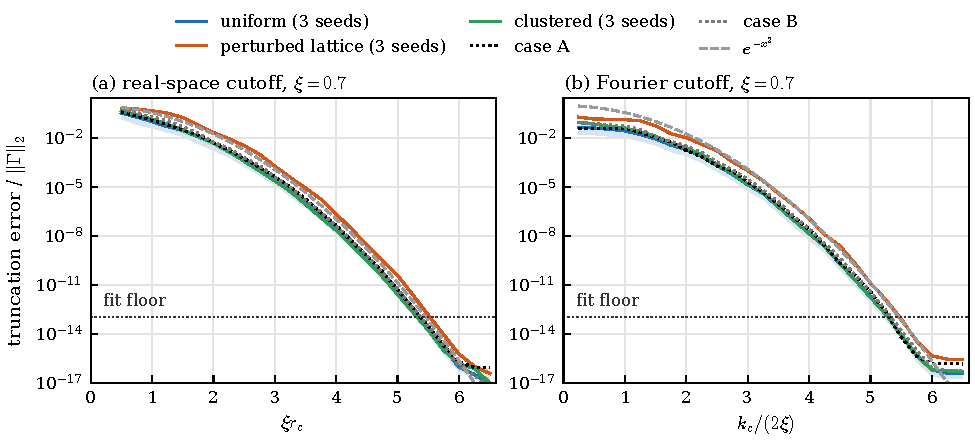
\includegraphics[width=\textwidth]{exp1_cutoffs.pdf}
\caption{Truncation errors at $\xi=0.7$, each with no other approximation. (a) Real-space cutoff; (b) Fourier cutoff
$\|\Gamma_L^{k_c}-\Gamma_L\|_2$. Both are normalized by $\|\Gamma\|_2$. Solid curves: median over three seeds of each
main-set family; bands: range over seeds; dotted: cases A and B; dashed: $e^{-x^2}$; horizontal dotted line: fit floor.
Below the fit floor the Fourier error levels off at the numerical floor of Appendix~\ref{app:exp-details}.}
\label{fig:exp-cutoffs}
\end{figure}

\paragraph{Mesh.}
At the T7 cutoff $k_c=5.74$ the long-range particle--mesh operator
$\widetilde\Gamma_h^L$ of Eq.~\eqref{eq:pm-graph} is compared with the
mesh-free sum $\Gamma_L^{k_c}$ over the same modes, so the difference is the
mesh error alone. The scan covers $p=3,\dots,8$, nine meshes from
$k_ch/\pi\approx0.91$--$0.99$ down to $0.23$--$0.25$, and eight grid shifts per mesh
(the unshifted grid and seven random global offsets), on cases A, B and the
main set (Fig.~\ref{fig:exp-mesh}a). On the four finest meshes above the fit
floor ($k_ch/\pi\approx0.23$--$0.50$) the median fitted slopes in $h$ are
$3.09$, $4.07$, $5.24$, $6.19$, $7.46$, $8.50$ for $p=3,\dots,8$
(Fig.~\ref{fig:exp-mesh}b); a repetition at the larger cutoff $s=5.5$ gives
$4.10$, $6.25$, $8.51$ for $p=4,6,8$. These slopes are consistent with the
$h^p$ law of Section~\ref{sec:pm}. On coarser meshes the fitted exponent is
$1.10$--$1.27\,p$, consistent with the factor $q^p$ of the leading alias, whose
local exponent approaches $p$ only as $h\to0$. A fit over finitely many meshes
does not establish the asymptotic order, and no asymptotic constant is
reported. Over the eight grid shifts the largest error is at most $1.30$
times the RMS.

In the exact off-grid decomposition of Eq.~\eqref{eq:pair-error}, evaluated
on the unshifted grid for $p=4,7$ and two meshes on cases A, B and one seed of
each main family, the linear terms $\alpha_i^*+\alpha_j$ carry
$0.996$--$1.003$ of the mesh error in the spectral norm, the quadratic term
$\alpha_i^*\alpha_j$ at most $0.9\%$, and $D_h$ at most $4.3\times10^{-9}$ of
it, as expected for ideal deconvolution. A diagnostic that kept only the
quadratic term would miss the mesh error almost entirely.

\begin{figure}[htbp]
\centering
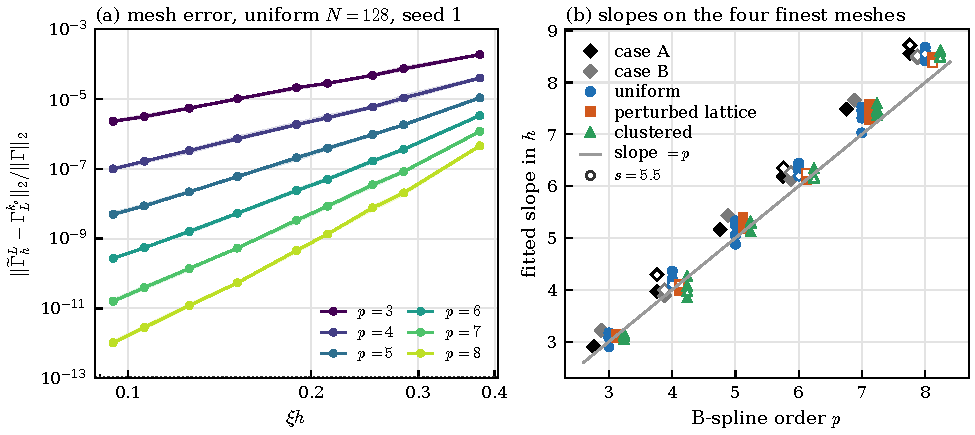
\includegraphics[width=\textwidth]{exp1_mesh.pdf}
\caption{Mesh error at $k_c=5.74$ ($s=4.1$, $\xi=0.7$). (a) $\|\widetilde\Gamma_h^L-\Gamma_L^{k_c}\|_2/\|\Gamma\|_2$ versus
$\xi h$ for the uniform configuration $N=128$, seed 1: RMS over eight grid shifts (points) and range over shifts (bands);
dotted: fit floor. (b) Fitted slopes in $h$ on the four finest meshes above the fit floor, one point per configuration and
$p$ (filled: $s=4.1$; open: $s=5.5$, five configurations); line: slope $p$.}
\label{fig:exp-mesh}
\end{figure}

\subsection{The complete production action}
\label{sec:exp-action}

The production code path (real-space pair loop, B-spline spreading,
FFT, multiplication by the influence function on $|\kk|\le k_c$, inverse
FFT, adjoint gathering and the degree correction) is applied to the $3N$ unit
vectors, giving $\widetilde\Gamma_h$ column by column, and to probe vectors.
The columns agree with an independent mode-space assembly to
$1.1\times10^{-15}$, and the separately measured terms
$\epsilon_S$, $\epsilon_F$, $\epsilon_{\mathrm{mesh}}$ of
Eq.~\eqref{eq:op-budget} add up to $1.2$--$2.0$ times the measured error.
Three quantities are kept apart: the relative operator error
$\|\widetilde\Gamma_h-\Gamma\|_2/\|\Gamma\|_2$, on which the sets were
accepted; the absolute operator error $\|\widetilde\Gamma_h-\Gamma\|_2$; and
the relative action error $\|(\widetilde\Gamma_h-\Gamma)X\|/\|\Gamma X\|$ for a
given vector $X$.

\paragraph{Relative operator error.}
Table~\ref{tab:exp-status} and Fig.~\ref{fig:exp-operator}a compare the
relative operator error with the tolerance for which each set was accepted.
T5 and T9 were tested on the 14 configurations of cases A, B, the main and the
check sets, T7 also on the 30 box-length configurations. Cases A and B meet
their tolerances, as selected. The other configurations do not all do so: T5
meets $10^{-5}$ on 10 of 14 configurations, with largest relative operator
error $1.2875\times10^{-5}$; T7 meets $10^{-7}$ on 39 of 44, with largest
$2.1056\times10^{-7}$; T9 meets $10^{-9}$ on 10 of 14, with largest
$2.5451\times10^{-9}$. The exceedances are at most a factor $2.55$. They occur
on the perturbed lattices for all three sets, and at T7 also on one uniform
box of the fixed-density set ($N=30$, $L=6$, seed 3; $1.40\times10^{-7}$),
which has the size, density and generator of case A and differs from it only
in the seed. The nominal tolerances are therefore not guaranteed beyond the
two configurations on which they were calibrated. For the production set T7
the measured statement is: on the 44 static configurations tested, the
relative operator error does not exceed $2.2\times10^{-7}$.

\begin{table}[htbp]
\centering
\small
\begin{tabular}{lllllll}
\toprule
set & tolerance & meets / tested & largest rel.\ error & absolute error & exceeding \\
\midrule
T5 & $10^{-5}$ & 10 / 14 & $1.2875\times10^{-5}$ & $7.7\times10^{-6}$--$3.3\times10^{-5}$ & lattices \\
T7 & $10^{-7}$ & 39 / 44 & $2.1056\times10^{-7}$ & $5.7\times10^{-8}$--$5.5\times10^{-7}$ & lattices, one uniform box \\
T9 & $10^{-9}$ & 10 / 14 & $2.5451\times10^{-9}$ & $1.3\times10^{-9}$--$7.1\times10^{-9}$ & lattices \\
\bottomrule
\end{tabular}
\caption{Relative operator error $\|\widetilde\Gamma_h-\Gamma\|_2/\|\Gamma\|_2$ against the tolerance for which the set was
accepted on cases A and B. ``Lattices'': the three perturbed lattices at $N=128$ and the one at $N=256$. Source:
\texttt{parameter\_set\_status.json}.}
\label{tab:exp-status}
\end{table}

Both the numerator and the denominator of the relative error depend on the
configuration (Fig.~\ref{fig:exp-operator}b). At T7 the absolute error varies
by about a factor ten over the 44 configurations, from $5.7\times10^{-8}$ to
$5.5\times10^{-7}$, and is largest for the densest fixed-$N$ boxes ($L=4$) and the clustered configurations.
$\|\Gamma\|_2$ is strongly influenced by close pairs, but not set by the
nearest pair alone: with $\theta(r)=e^{-\kappa r}/r$, the ratio
$\|\Gamma\|_2/\theta(d_{\min})$ is $2.0$--$4.1$, whereas an isolated pair gives
$2$. Every configuration that exceeds its tolerance has a small norm
($0.72$--$0.94$ for the lattices, $1.50$ for the uniform box) and a moderate
absolute error. A small norm is not sufficient, however: the fixed-$N$ box
with $L=16$, seed 1, has $\|\Gamma\|_2=1.34$ and meets $10^{-7}$ because its
absolute error is smaller.

\begin{figure}[htbp]
\centering
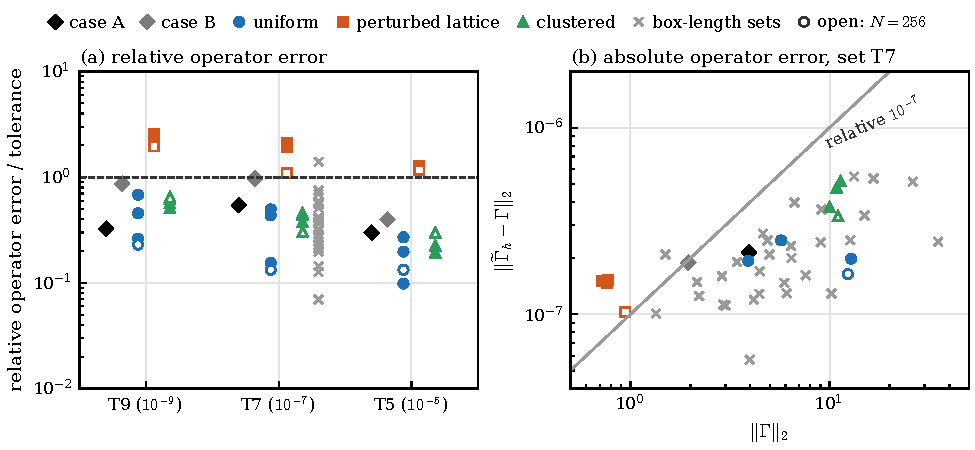
\includegraphics[width=\textwidth]{exp1_operator.pdf}
\caption{The production operator against the reference, 44 static configurations, one point per configuration. (a)
Relative operator error divided by the tolerance for which the set was accepted on cases A and B; dashed: tolerance.
Box-length sets were tested with T7 only. (b) Absolute operator error against $\|\Gamma\|_2$ at T7; the line marks a
relative error $10^{-7}$.}
\label{fig:exp-operator}
\end{figure}

\paragraph{Error budget.}
For cases A, B and the main set at T7 the mesh term is the largest
($\epsilon_{\mathrm{mesh}}\le1.5\times10^{-7}$ relative), followed by the
real-space and Fourier truncations ($\le1.05\times10^{-7}$ and
$\le7\times10^{-8}$, largest for the lattices). The real-space term is the
largest for the $N=256$ lattice and for five boxes at the smallest realised
$k_ch/\pi=0.61$.

\paragraph{Action on probe vectors.}
The probes are sixteen mean-free Gaussian vectors, the modes of the lowest
nonzero wave number $2\pi/L$ along each axis (longitudinal and transverse,
projected onto $\Range\Pi$), and the translations
(Fig.~\ref{fig:exp-probes}a). A relative action error can exceed the relative
operator error by the factor $\|\Gamma\|_2\|X\|/\|\Gamma X\|$, which is large
for slowly varying vectors: $\|\Gamma X\|/(\|\Gamma\|_2\|X\|)$ is as small as
$2.5\times10^{-2}$ (longitudinal) and $1.1\times10^{-2}$ (transverse) on cases A,
B and the main set, where these probes exceed their configuration's relative
operator error by factors up to $14$ and $18$. Meeting the operator tolerance
therefore does not imply meeting it for every action. At T7, all 39
configurations with relative operator error at most $10^{-7}$ have a
transverse probe with relative action error above $10^{-7}$; 32 have such a
longitudinal and 21 such a Gaussian probe. Among these 39, the largest
relative action errors are $2.2$, $3.7$ and $4.5$ times $10^{-7}$ (Gaussian,
longitudinal, transverse). At T5 and T9, 8 and 10 of the 10 configurations
within the operator tolerance have a transverse probe above it, by up to
factors $2.5$ and $4.9$. The production operator annihilates the translations
exactly in floating point, because the degree correction cancels the constant
field term by term; the reference residual is at most $1.9\times10^{-16}$.

\paragraph{Symmetry and spectrum.}
$\widetilde\Gamma_h$ is symmetric to $1.0\times10^{-16}$ (relative Frobenius
norm). The smallest eigenvalue of $\Gamma$ on $\Range\Pi$ ranges from
$7.9\times10^{-4}$ to $1.92$ over the configurations, and
$\lambda_{\min}(\widetilde\Gamma_h|_{\Range\Pi})$ differs from it by at most
$4.2\times10^{-5}$ (T5), $1.6\times10^{-6}$ (T7) and $2.6\times10^{-8}$ (T9),
relative. In every one of the 72 tested pairs of configuration and set,
$\|\widetilde\Gamma_h-\Gamma\|_2<\lambda_{\min}(\Gamma|_{\Range\Pi})$, so the
raw particle--mesh graph is positive semidefinite on these configurations
without stabilization; the observed shift of the smallest eigenvalue is a
median $13\%$ and at most $41\%$ of $\|\widetilde\Gamma_h-\Gamma\|_2$. These are
observations on finitely many configurations, not a general positivity
result.

\paragraph{Box length and density.}
At T7 the two box-length sets separate different effects
(Fig.~\ref{fig:exp-probes}b; medians over three seeds). At fixed $N=64$ the
density and $\kappa L$ change together; the absolute error falls from
$5.3\times10^{-7}$ ($L=4$, density $1$) to $1.0\times10^{-7}$ ($L=16$, density
$0.016$), with all three budget terms decreasing, though not monotonically.
At fixed density $N$ grows with $L$, and the absolute error is
$2.1\times10^{-7}$, $1.1\times10^{-7}$, $2.5\times10^{-7}$ and
$2.5\times10^{-7}$ for $L=6$, $8$, $10$, $12$, a change of at most a factor
$2.2$. In both sets the dip at $L=8$ coincides with the smaller realised
$k_ch/\pi=0.61$ caused by rounding $M$ to a smooth size; for $p=7$ the $h^p$
trend predicts a factor $(0.61/0.68)^7\approx0.45$ in the mesh term. This was
not rerun at matched $k_ch/\pi$, and the set does not separate the effect of
$L$ from that of $N$ and the particle arrangement.

\begin{figure}[htbp]
\centering
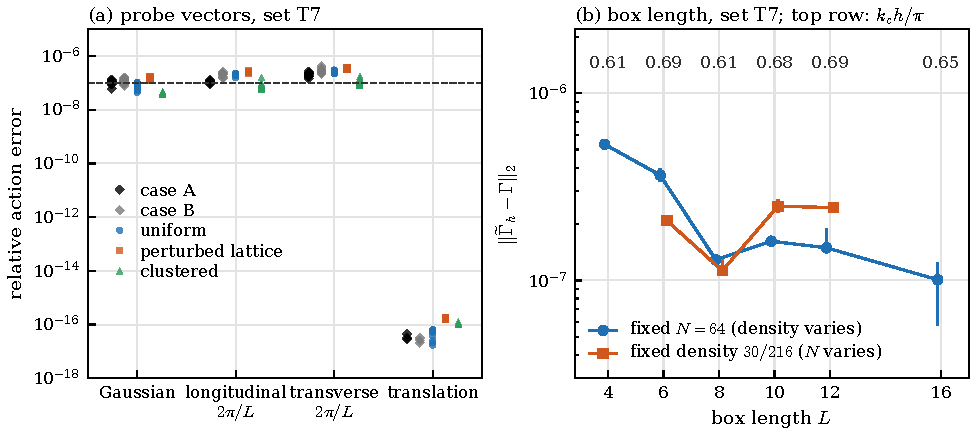
\includegraphics[width=\textwidth]{exp1_probes_box.pdf}
\caption{(a) Relative action errors $\|(\widetilde\Gamma_h-\Gamma)X\|/\|\Gamma X\|$ of probe vectors at T7 through the
production action, cases A, B and the main set; dashed: $10^{-7}$. For the translations $t\in\cT$, where $\Gamma t=0$, the
quantity shown is $\|(\widetilde\Gamma_h-\Gamma)t\|/(\|\Gamma\|_2\|t\|)$, which equals the reference residual because
$\widetilde\Gamma_ht=0$ exactly. (b) Absolute operator error at T7 against box length; points: median over three seeds,
bars: range; top row: realised $k_ch/\pi$, which is the same in both sets at equal $L$.}
\label{fig:exp-probes}
\end{figure}

\subsection{Summary}
\label{sec:exp-summary}

On static configurations with $\kappa=1$ and $N\le256$ the experiment
establishes the following. The dense reference converges numerically under
image refinement and is reproduced by the split construction to
$1.1\times10^{-15}$. Both truncations decay at the Gaussian rate over the
fitted window, and the mesh error has slopes consistent with $h^p$ on the
finest meshes, carried almost entirely by the linear alias terms. The
production action reproduces the separately measured budget, is symmetric,
annihilates the translations exactly and remained positive semidefinite in
every tested case. The parameter sets calibrated on cases A and B do not meet
their nominal relative tolerance on every configuration: 4 of 14 (T5), 5 of
44 (T7) and 4 of 14 (T9) exceed it, by up to a factor $2.55$. Even where the
operator tolerance is met, relative action errors of slowly varying vectors
exceed it by up to a factor $4.9$. Parameters therefore have to be checked on
configurations representative of their use, and the action on slow modes has
to be checked separately from the operator norm.

\section{Conclusion}
\label{sec:conclusion}

Sections~\ref{sec:kernel}--\ref{sec:error} address the
consequences of the screened longitudinal Ewald long-range kernel for the
particle graph and its PPPM discretization. The analysis rests on two
properties: the real-space long-range pair kernel is pointwise positive
semidefinite, and its Fourier multiplier has Gaussian decay
$\mathcal{O}(e^{-k^2/(4\xi^2)})$. The Fourier multiplier itself need not be positive
semidefinite; positivity of the exact friction follows instead from the
pointwise semidefinite pair kernel and the graph degree-minus-weight
structure.

Finite reciprocal and particle--mesh approximations preserve symmetry and
the translation nullspace when adjoint spreading/gathering and a common
degree-minus-weight construction are used. Their operator error is
controlled by the complete pair-response discrepancy. For ideal
particle--mesh deconvolution, the leading mesh error is generated by the
linear off-grid alias cross terms and satisfies
\begin{equation}
\epsilon_{\mathrm{mesh}}=\mathcal{O}(h^p)
\end{equation}
for a B-spline assignment of order $p$. The resulting practical error model
is
\begin{equation}
\epsilon_{\mathrm{op}}
\lesssim
C_Ee^{-s^2}
+
C_M(\xi h)^p,
\qquad
s=\xi r_c=\frac{k_c}{2\xi}.
\end{equation}
A useful initial choice is
\begin{equation}
s=\sqrt{\log(2/\mathrm{tol})},
\qquad
r_c=\frac{s}{\xi},
\qquad
k_c=2\xi s,
\end{equation}
followed by a mesh chosen from the measured envelope of $C_M$ and a Nyquist
safety condition. Accuracy is certified by a complete pair-response
operator bound, while
\begin{equation}
\epsilon_{\mathrm{op}}<\lambda_*
\end{equation}
provides a sufficient, although conservative, certificate that the raw
discrete graph remains positive semidefinite.

The operator experiment of Section~\ref{sec:experiments}, on static
configurations with $\kappa=1$ and $N\le256$, supports the components of this
error model: both truncations decay at the Gaussian rate, the mesh error has
slopes consistent with $h^p$ on the finest meshes and is carried by the linear
alias terms, and the production action reproduces the separately measured
budget, preserves symmetry and the translation null space, and remained
positive semidefinite in every tested case. It also shows the limits of a
calibration on few configurations. Parameter sets accepted for the relative
tolerances $10^{-5}$, $10^{-7}$ and $10^{-9}$ on two boxes met them on 10 of 14,
39 of 44 and 10 of 14 configurations, respectively, with largest relative
operator errors $1.2875\times10^{-5}$, $2.1056\times10^{-7}$ and
$2.5451\times10^{-9}$; for the set T7 the measured statement is a relative
operator error of at most $2.2\times10^{-7}$ on the 44 configurations tested.
Relative action errors on slowly varying vectors can exceed the relative
operator error severalfold. These are finite-sample observations; positivity
and the observed slopes are not general results.

\appendix

\section{Gaussian-scale representation}
\label{app:gauss-scale}

This appendix proves Proposition~\ref{prop:gauss-scale}.

\paragraph{Gaussian representations of the two factors.}
We factor the scalar part of the kernel as
\begin{equation}
\frac{e^{-\kappa r}}{r^3}
=
\frac{e^{-\kappa r}}{r}\cdot\frac{1}{r^2}
\end{equation}
and represent each factor as a superposition of Gaussians in $r$.
For the Yukawa factor we use the standard representation
\begin{equation}
\frac{e^{-\kappa r}}{r}
=
\frac{1}{\sqrt{\pi}}
\int_0^\infty
t^{-1/2}
e^{-\kappa^2/(4t)}
e^{-t r^2}\,dt,
\end{equation}
which is the integral
$\int_0^\infty t^{-1/2}e^{-at-b/t}\,dt=\sqrt{\pi/a}\,e^{-2\sqrt{ab}}$,
$a,b>0$, evaluated at $a=r^2$ and $b=\kappa^2/4$. For the second factor,
\begin{equation}
\frac{1}{r^2}
=
\int_0^\infty e^{-u r^2}\,du .
\end{equation}
Thus the Gaussian-scale weights of the two factors are
$\pi^{-1/2}t^{-1/2}e^{-\kappa^2/(4t)}$ and the constant $1$.

\paragraph{Convolution of the weights.}
Multiplying the two representations, the Gaussians combine as
$e^{-t r^2}e^{-u r^2}=e^{-(t+u)r^2}$, so the product is again a
superposition of Gaussians, with scale $s=t+u$. Its weight is the
Laplace convolution of the two weights. Explicitly, by Tonelli's
theorem, since all integrands are nonnegative,
\begin{align}
\frac{e^{-\kappa r}}{r^3}
&=
\frac{1}{\sqrt{\pi}}
\int_0^\infty
\int_0^\infty
t^{-1/2}
e^{-\kappa^2/(4t)}
e^{-(t+u) r^2}\,du\,dt
\\
&=
\frac{1}{\sqrt{\pi}}
\int_0^\infty
\int_t^\infty
t^{-1/2}
e^{-\kappa^2/(4t)}
e^{-s r^2}\,ds\,dt
\\
&=
\int_0^\infty
\left[
\frac{1}{\sqrt{\pi}}
\int_0^s
t^{-1/2}
e^{-\kappa^2/(4t)}\cdot 1\,dt
\right]
e^{-s r^2}\,ds
\\
&=
\int_0^\infty
\rho_\kappa(s)e^{-s r^2}\,ds,
\end{align}
where the second line substitutes $s=t+u$ in the inner integral and the
third exchanges the order of integration over $0<t<s<\infty$. The
bracket is the convolution
$\int_0^s(\pi^{-1/2}t^{-1/2}e^{-\kappa^2/(4t)})\cdot1\,dt$ of the
Yukawa weight with the constant weight of $1/r^2$. Multiplying by
$\rr\rr^{\mathsf T}$ and using
\begin{equation}
K_\kappa(\rr)
=
e^{-\kappa r}\frac{\rr\rr^{\mathsf T}}{r^3}
\end{equation}
gives Eq.~\eqref{eq:gauss-scale}.

\paragraph{Closed form of the weight.}
Let $\varphi(s)$ denote the right-hand side of the second equality in
Eq.~\eqref{eq:rho}. Differentiation gives
\begin{align}
\frac{d}{ds}
\left[
\frac{2\sqrt{s}}{\sqrt{\pi}}e^{-\kappa^2/(4s)}
\right]
&=
\frac{1}{\sqrt{\pi}}
\left(
s^{-1/2}+\frac{\kappa^2}{2}s^{-3/2}
\right)
e^{-\kappa^2/(4s)},
\\
\frac{d}{ds}
\left[
\kappa\left[\erf\!\left(\frac{\kappa}{2\sqrt s}\right)-1\right]
\right]
&=
-\frac{\kappa^2}{2\sqrt{\pi}}\,s^{-3/2}e^{-\kappa^2/(4s)},
\end{align}
so $\varphi'(s)=\pi^{-1/2}s^{-1/2}e^{-\kappa^2/(4s)}$. Since
$\varphi(s)\to0$ as $s\to0^+$, $\varphi$ coincides with the integral
in Eq.~\eqref{eq:rho}.

\paragraph{Properties of the weight.}
The integrand in Eq.~\eqref{eq:rho} is positive and bounded by
$\pi^{-1/2}t^{-1/2}$. Hence $\rho_\kappa$ is positive and nondecreasing
on $(0,\infty)$, and
\begin{equation}
\label{eq:rho-bound}
\rho_\kappa(s)\le\frac{2\sqrt{s}}{\sqrt{\pi}}.
\end{equation}
In particular, $\rho_\kappa(\xi^2)>0$.

\section{Closed-form real-space coefficients}
\label{app:closed-form}

Let
\begin{equation}
z=\frac{\kappa}{2\xi},
\end{equation}
and define
\begin{equation}
c_{\kappa,\xi}
=
\rho_\kappa(\xi^2)
=
\frac{2\xi}{\sqrt{\pi}}e^{-z^2}
+
\kappa\left[\erf(z)-1\right].
\end{equation}
The long-range scalar coefficient can be written as
\begin{equation}
\theta_L(r)
=
Y_\kappa^L(r)
-
c_{\kappa,\xi}e^{-\xi^2r^2},
\end{equation}
where
\begin{equation}
Y_\kappa^L(r)
=
\frac{1}{2r}
\left[
e^{-\kappa r}
\erfc\!\left(z-\xi r\right)
-
e^{\kappa r}
\erfc\!\left(z+\xi r\right)
\right].
\end{equation}
Similarly,
\begin{equation}
\theta_S(r)
=
Y_\kappa^S(r)
+
c_{\kappa,\xi}e^{-\xi^2r^2},
\end{equation}
with
\begin{equation}
Y_\kappa^S(r)
=
\frac{1}{2r}
\left[
e^{-\kappa r}
\erfc\!\left(\xi r-z\right)
+
e^{\kappa r}
\erfc\!\left(\xi r+z\right)
\right].
\end{equation}
Since
\begin{equation}
Y_\kappa^S(r)+Y_\kappa^L(r)
=
\frac{e^{-\kappa r}}{r},
\end{equation}
the identity \(K_\kappa^S+K_\kappa^L=K_\kappa\) follows immediately.

\section{Localization estimates}
\label{app:localization}

This appendix proves Proposition~\ref{prop:localization} and
Eq.~\eqref{eq:tails}.

\paragraph{Real-space decay.}
Fix $r>0$. Since $r^2e^{-sr^2}=-\frac{d}{ds}e^{-sr^2}$, integration by parts
in
\begin{equation}
\theta_S(r)
=
r^2\int_{\xi^2}^{\infty}
\rho_\kappa(s)e^{-sr^2}\,ds
\end{equation}
gives
\begin{equation}
\label{eq:thetaS-ibp}
\theta_S(r)
=
\rho_\kappa(\xi^2)e^{-\xi^2r^2}
+
\int_{\xi^2}^{\infty}
\rho_\kappa'(s)e^{-sr^2}\,ds .
\end{equation}
The boundary term at infinity vanishes: by Eq.~\eqref{eq:rho-bound},
$0\le\rho_\kappa(s)e^{-sr^2}\le2\pi^{-1/2}\sqrt{s}\,e^{-sr^2}\to0$ as
$s\to\infty$. By Appendix~\ref{app:gauss-scale},
\begin{equation}
\rho_\kappa'(s)
=
\frac{1}{\sqrt{\pi s}}\,e^{-\kappa^2/(4s)},
\end{equation}
so $0\le\rho_\kappa'(s)\le(\sqrt{\pi}\,\xi)^{-1}$ for $s\ge\xi^2$. Inserting
this bound in the last integral of Eq.~\eqref{eq:thetaS-ibp} and using
$\int_{\xi^2}^\infty e^{-sr^2}\,ds=e^{-\xi^2r^2}/r^2$ gives
\begin{equation}
0
\le
\theta_S(r)-\rho_\kappa(\xi^2)e^{-\xi^2r^2}
\le
\frac{e^{-\xi^2r^2}}{\sqrt{\pi}\,\xi r^2} .
\end{equation}
Hence, for fixed $\kappa,\xi>0$,
\begin{equation}
\theta_S(r)
=
e^{-\xi^2r^2}
\left[\rho_\kappa(\xi^2)+\mathcal O(r^{-2})\right],
\qquad r\to\infty .
\end{equation}
Since $\rho_\kappa(\xi^2)>0$, this gives
$\theta_S(r)\sim\rho_\kappa(\xi^2)e^{-\xi^2r^2}$, and
$K_\kappa^S(\rr)=\theta_S(r)\PP(\rr)$ yields Eq.~\eqref{eq:KS-asym}.

\paragraph{Fourier transform.}
For a Gaussian,
\begin{equation}
\mathcal F[e^{-sr^2}]
=
\left(\frac{\pi}{s}\right)^{3/2}
e^{-k^2/(4s)}.
\end{equation}
With the convention used here, multiplication by $r_a$ corresponds to
$i\,\partial/\partial k_a$ in Fourier space, so
$\mathcal F[r_ar_b e^{-sr^2}]
=-\partial_{k_a}\partial_{k_b}\mathcal F[e^{-sr^2}]$. Since
$\partial_{k_a}\partial_{k_b}e^{-k^2/(4s)}
=\bigl(k_ak_b/(4s^2)-\delta_{ab}/(2s)\bigr)e^{-k^2/(4s)}$,
\begin{equation}
\mathcal F[
r_a r_b e^{-sr^2}
]
=
\left(\frac{\pi}{s}\right)^{3/2}
e^{-k^2/(4s)}
\left[
\frac{\delta_{ab}}{2s}
-
\frac{k_a k_b}{4s^2}
\right].
\end{equation}
Integrating against $\rho_\kappa(s)$ over $(0,\xi^2)$, which is permitted
because $\rho_\kappa(s)s^{-7/2}$ is integrable near $s=0$, gives
Eq.~\eqref{eq:KL-fourier} with the stated $A_{\kappa,\xi}$ and
$B_{\kappa,\xi}$. Differentiating $A_{\kappa,\xi}$ under the integral
sign, $\partial_k e^{-k^2/(4s)}=-(k/(2s))e^{-k^2/(4s)}$, gives
\begin{equation}
B_{\kappa,\xi}(k)
=
\frac{1}{k}
\frac{d}{dk}A_{\kappa,\xi}(k),
\qquad
k>0.
\end{equation}

\paragraph{Endpoint asymptotics.}
Let $k>0$ and, for $m\in\{5/2,7/2\}$,
\begin{equation}
I_m(k)
=
\int_0^{\xi^2}
\rho_\kappa(s)s^{-m}e^{-k^2/(4s)}\,ds,
\end{equation}
so that $A_{\kappa,\xi}(k)=\tfrac{\pi^{3/2}}{2}I_{5/2}(k)$ and
$B_{\kappa,\xi}(k)=-\tfrac{\pi^{3/2}}{4}I_{7/2}(k)$. Since
\begin{equation}
\frac{d}{ds}e^{-k^2/(4s)}
=
\frac{k^2}{4s^2}e^{-k^2/(4s)},
\end{equation}
we write $\rho_\kappa(s)s^{-m}=s^{-2}\,\rho_\kappa(s)s^{2-m}$ and integrate
by parts, first on $[\varepsilon,\xi^2]$ and then letting
$\varepsilon\to0^+$:
\begin{equation}
\label{eq:Im-ibp}
I_m(k)
=
\frac{4\rho_\kappa(\xi^2)\xi^{4-2m}}{k^2}
e^{-k^2/(4\xi^2)}
-
\frac{4}{k^2}
\int_0^{\xi^2}
\frac{d}{ds}\!\left[\rho_\kappa(s)s^{2-m}\right]
e^{-k^2/(4s)}\,ds .
\end{equation}
The boundary term at $s=0$ vanishes: by Eq.~\eqref{eq:rho-bound},
\begin{equation}
0
\le
\rho_\kappa(s)s^{2-m}e^{-k^2/(4s)}
\le
\frac{2}{\sqrt{\pi}}\,s^{5/2-m}e^{-k^2/(4s)}
\longrightarrow0,
\qquad s\to0^+,
\end{equation}
because the exponential factor decays faster than any power of $s$.

To bound the remaining integral we use
$\rho_\kappa'(s)\le\pi^{-1/2}s^{-1/2}$ and
Eq.~\eqref{eq:rho-bound}. For $0<s\le\xi^2$,
\begin{equation}
\begin{aligned}
\left|
s^2\frac{d}{ds}\!\left[\rho_\kappa(s)s^{2-m}\right]
\right|
&=
\left|
s^{4-m}\rho_\kappa'(s)+(2-m)s^{3-m}\rho_\kappa(s)
\right|
\\
&\le
\frac{1+2|m-2|}{\sqrt{\pi}}\,s^{7/2-m}
\le
\frac{1+2|m-2|}{\sqrt{\pi}}\,\xi^{7-2m},
\end{aligned}
\end{equation}
where the last step uses $7/2-m\ge0$. Hence, with
$\int_0^{\xi^2}s^{-2}e^{-k^2/(4s)}\,ds=(4/k^2)e^{-k^2/(4\xi^2)}$,
\begin{equation}
\left|
\frac{4}{k^2}
\int_0^{\xi^2}
\frac{d}{ds}\!\left[\rho_\kappa(s)s^{2-m}\right]
e^{-k^2/(4s)}\,ds
\right|
\le
\frac{16\,(1+2|m-2|)\,\xi^{7-2m}}{\sqrt{\pi}\,k^4}
e^{-k^2/(4\xi^2)} ,
\end{equation}
which is $\mathcal O\bigl(k^{-4}e^{-k^2/(4\xi^2)}\bigr)$. The same bound
shows that the integral in Eq.~\eqref{eq:Im-ibp} converges absolutely, which
justifies the limit $\varepsilon\to0^+$. Since $\rho_\kappa(\xi^2)>0$,
\begin{equation}
I_m(k)
=
\frac{4\rho_\kappa(\xi^2)\xi^{4-2m}}{k^2}
e^{-k^2/(4\xi^2)}
\left[1+\mathcal O(k^{-2})\right],
\qquad k\to\infty .
\end{equation}

With $m=5/2$ and $m=7/2$,
\begin{align}
A_{\kappa,\xi}(k)
&=
\frac{2\pi^{3/2}}{\xi k^2}\rho_\kappa(\xi^2)e^{-k^2/(4\xi^2)}
\left[1+\mathcal O(k^{-2})\right],
\\
k^2B_{\kappa,\xi}(k)
&=
-\frac{\pi^{3/2}}{\xi^3}\rho_\kappa(\xi^2)e^{-k^2/(4\xi^2)}
\left[1+\mathcal O(k^{-2})\right].
\end{align}
Thus
\begin{equation}
\frac{A_{\kappa,\xi}(k)}{k^2B_{\kappa,\xi}(k)}
=
-\frac{2\xi^2}{k^2}\left[1+\mathcal O(k^{-2})\right],
\qquad
\lambda_\parallel(k)
=
A_{\kappa,\xi}(k)+k^2B_{\kappa,\xi}(k)
=
k^2B_{\kappa,\xi}(k)\left[1+\mathcal O(k^{-2})\right],
\end{equation}
which is Eq.~\eqref{eq:lambda-par-asym}; in particular $\lambda_\parallel(k)<0$ for
all sufficiently large $k$. The eigenvalues of the symmetric matrix
$\widehat K_\kappa^L(\kk)$ are $\lambda_\perp(k)=A_{\kappa,\xi}(k)>0$
(twice) and $\lambda_\parallel(k)$, so its spectral norm is
$\max\{\lambda_\perp(k),|\lambda_\parallel(k)|\}$. Because
$\lambda_\perp(k)/|\lambda_\parallel(k)|=\mathcal O(k^{-2})$, the norm equals
$|\lambda_\parallel(k)|$ for large $k$, which gives Eq.~\eqref{eq:KL-decay}.

\paragraph{Tail quantities.}
Since $\|\theta_S(r)\PP(\rr)\|_2=\theta_S(r)$, spherical coordinates give
\begin{equation}
E_S(r_c)
=
4\pi
\int_{r_c}^{\infty}
r^2\theta_S(r)\,dr,
\qquad
E_F(k_c)
=
\frac{1}{2\pi^2}
\int_{k_c}^{\infty}
k^2
\left\|
\widehat K_\kappa^L(k)
\right\|_2\,dk.
\end{equation}
For $c>0$, integration by parts gives
\begin{equation}
\int_{x_0}^{\infty}x^2e^{-cx^2}\,dx
=
\frac{x_0}{2c}e^{-cx_0^2}
+
\frac{1}{2c}\int_{x_0}^{\infty}e^{-cx^2}\,dx,
\end{equation}
and the last integral is at most $e^{-cx_0^2}/(2cx_0)$. Hence
\begin{equation}
\int_{r_c}^{\infty}
r^2e^{-\xi^2r^2}\,dr
\sim
\frac{r_c}{2\xi^2}
e^{-\xi^2r_c^2},
\qquad
\int_{k_c}^{\infty}
k^2e^{-k^2/(4\xi^2)}\,dk
\sim
2\xi^2 k_c
e^{-k_c^2/(4\xi^2)}.
\end{equation}
Because the integrands are asymptotically equivalent to
$\rho_\kappa(\xi^2)e^{-\xi^2r^2}$ and
$(\pi^{3/2}/\xi^3)\rho_\kappa(\xi^2)e^{-k^2/(4\xi^2)}$, respectively, the tails inherit these
rates:
\begin{equation}
E_S(r_c)
\sim
4\pi\rho_\kappa(\xi^2)
\frac{r_c}{2\xi^2}
e^{-\xi^2r_c^2},
\qquad
E_F(k_c)
\sim
\frac{\rho_\kappa(\xi^2)}{2\sqrt{\pi}\,\xi^3}\,
2\xi^2 k_c
e^{-k_c^2/(4\xi^2)},
\end{equation}
which is Eq.~\eqref{eq:tails}.

\section{Pair-response operator bounds}
\label{app:pair-response}

\begin{lemma}[Pair-response perturbation]
\label{lem:pair-response}
Let $\Gamma$ and $\Gamma'$ be built by the degree-minus-weight
construction, $(\Gamma X)_i=\sum_{j\ne i}K_{ij}(x_i-x_j)$, from pair
responses $K_{ij}$ and $K'_{ij}$, and let $E_{ij}=K'_{ij}-K_{ij}$. If
$E_{ij}=E_{ji}=E_{ij}^{\mathsf T}$ for all $i\ne j$, then
\begin{equation}
\|\Gamma'-\Gamma\|_2
\le
2\max_i\sum_{j\ne i}\|E_{ij}\|_2 .
\end{equation}
\end{lemma}

\begin{proof}
The difference $\Gamma'-\Gamma$ is symmetric, and pairing the $(i,j)$ and
$(j,i)$ terms gives
\begin{equation}
X^{\mathsf T}(\Gamma'-\Gamma)X
=
\frac12\sum_{i\ne j}(x_i-x_j)^{\mathsf T}E_{ij}(x_i-x_j).
\end{equation}
Using $|x_i-x_j|^2\le2|x_i|^2+2|x_j|^2$ and the symmetry in $i,j$,
\begin{equation}
\left|X^{\mathsf T}(\Gamma'-\Gamma)X\right|
\le
2\sum_i|x_i|^2\sum_{j\ne i}\|E_{ij}\|_2
\le
2\max_i\sum_{j\ne i}\|E_{ij}\|_2\,|X|^2 .
\end{equation}
For a symmetric operator the spectral norm is the supremum of the
quadratic form over unit vectors.
\end{proof}

The hypothesis holds for every even, pointwise symmetric pair kernel. It
also holds for the particle--mesh response, because an even, real-symmetric
influence function makes each block of $W_h$ real and symmetric and
$(W_h)_{ij}=(W_h)_{ji}$. Lemma~\ref{lem:pair-response} with
$E_{ij}=R_{k_c}(q_i-q_j)$ gives Eq.~\eqref{eq:trunc-bound}. Since
$|e^{i\kk\cdot\rr}|=1$, every term satisfies
$\|R_{k_c}(\rr)\|_2\le V^{-1}\sum_{|\kk|>k_c}\|\widehat K_\kappa^L(\kk)\|_2$,
and the sum over $j\ne i$ has $N-1$ terms, which gives
Eq.~\eqref{eq:trunc-pessimistic}. Lemma~\ref{lem:pair-response} with
$E_{ij}=K^h_{ij}-K_{ij}$ gives Eq.~\eqref{eq:op-bound}.

\begin{proof}[Proof of Proposition~\ref{prop:stabilized}]
Both terms in Eq.~\eqref{eq:stabilized} are symmetric. Since
$\widetilde\Gamma_h$ has zero block-row sums, it annihilates $\cT$, and by
symmetry it maps $\Range\Pi=\cT^\perp$ into itself. Hence
$\Gamma_h t=\widetilde\Gamma_h t+\delta_h\Pi t=0$ for $t\in\cT$. For
arbitrary $X$, write $Y=\Pi X$. Then
\begin{equation}
X^{\mathsf T}\Gamma_hX
=
Y^{\mathsf T}\widetilde\Gamma_hY+\delta_h|Y|^2
\ge
\left(
\lambda_{\min}\bigl(\widetilde\Gamma_h|_{\Range\Pi}\bigr)+\delta_h
\right)|Y|^2
\ge0
\end{equation}
by the choice of $\delta_h$. Finally,
$\|\Gamma_h-\Gamma\|_2\le\|\widetilde\Gamma_h-\Gamma\|_2+\delta_h\|\Pi\|_2
\le\epsilon_{\mathrm{op}}+\delta_h$ by Eq.~\eqref{eq:op-bound} and
$\|\Pi\|_2=1$.
\end{proof}

\section{Particle--mesh alias response}
\label{app:alias}

\paragraph{Single-mode pair response.}
Spreading a particle at $q$ onto the mesh and taking the discrete Fourier
transform produces, for a retained mode $\kk$, the deposited amplitude
$S_h(\kk,q)$: sampling the window on the mesh folds all aliases
$\kk_n$ onto $\kk$. Because the assignment window is real and even,
$\widehat W_h$ is real, and gathering the field of mode $\kk$ at $q_i$
produces the factor $\overline{S_h(\kk,q_i)}$. Hence the contribution of
mode $\kk$ to $(W_h)_{ij}$ is proportional to
\begin{equation}
\overline{S_h(\kk,q_i)}\,G_h(\kk)\,S_h(\kk,q_j)
=
H_h(\kk)\,e^{i\kk\cdot(q_i-q_j)}
\left(1+\alpha_i^*\right)\left(1+\alpha_j\right),
\end{equation}
with the same normalization as the exact contribution
$\widehat K_\kappa^L(\kk)e^{i\kk\cdot(q_i-q_j)}$. Subtracting the exact
contribution and expanding the product gives Eq.~\eqref{eq:pair-error}.

\paragraph{B-spline alias ratio.}
Write $x_\ell=k_\ell h/2$. The $\ell$-th component of $\kk_n$ satisfies
$(\kk_n)_\ell h/2=x_\ell+\pi n_\ell$, and
$\sin(x_\ell+\pi n_\ell)=(-1)^{n_\ell}\sin x_\ell$. Therefore
\begin{equation}
\left|
\frac{\widehat W_h(\kk_n)}
{\widehat W_h(\kk)}
\right|
=
\prod_{\ell:n_\ell\ne0}
\left|
\frac{k_\ell h/2}
{k_\ell h/2+\pi n_\ell}
\right|^p.
\end{equation}
For a mode resolved by the mesh, $|x_\ell|\le\pi/2$, so
$|x_\ell+\pi n_\ell|\ge\pi|n_\ell|/2$ and each factor is at most
$(h|k_\ell|/\pi)^p|n_\ell|^{-p}$, where $h|k_\ell|/\pi\le1$ and
$|k_\ell|\le|\kk|$. Every $n\ne0$ has at least one nonzero component, so
the product of the factors $(h|k_\ell|/\pi)^p$ is at most
$(h|\kk|/\pi)^p$ and
\begin{equation}
|\alpha_h(\kk,q)|
\le
\left(\frac{h|\kk|}{\pi}\right)^p
\sum_{n\ne0}\ \prod_{\ell:n_\ell\ne0}|n_\ell|^{-p}
=
\left[
\left(1+2\sum_{m=1}^\infty m^{-p}\right)^3-1
\right]
\left(\frac{h|\kk|}{\pi}\right)^p,
\end{equation}
uniformly in $q$. The series converges for $p\ge2$, which gives
$\alpha_h(\kk,q)=\mathcal{O}((h|\kk|)^p)$.

\paragraph{Mesh law.}
For ideal deconvolution, $D_h=0$, and the bound on $\alpha_h$ gives, for
each pair,
\begin{equation}
\|E^h_{ij}\|_2
\lesssim
\frac1V\sum_{|\kk|\le k_c}
\|\widehat K_\kappa^L(\kk)\|_2
\left[(h|\kk|)^p+(h|\kk|)^{2p}\right],
\end{equation}
with a constant depending only on $p$. Summing over $j\ne i$ multiplies the
bound by $N-1$. The lattice sum
$V^{-1}\sum_{\kk}|\kk|^p\|\widehat K_\kappa^L(\kk)\|_2$ is a Riemann sum
for $M_p(\kappa,\xi)$ and is finite by the Gaussian decay in
Eq.~\eqref{eq:KL-decay}. Since $h|\kk|\le\sqrt3\,\pi$ on the resolved
modes, the $h^{2p}$ term is subdominant, which gives Eq.~\eqref{eq:mesh-law} for a fixed
configuration and cutoff.

\section{Finite-time thermostat}
\label{app:thermostat}

\paragraph{Exact covariance.}
For frozen positions, consider the Ornstein--Uhlenbeck dynamics
\begin{equation}
dp
=
-\frac1m\Gamma_h p\,dt
+
\left(2\beta^{-1}\Gamma_h\right)^{1/2}dW_t,
\end{equation}
where $W_t$ is a standard Wiener process. Over a step of length $\Delta t$,
the solution is $p(\Delta t)=R_{\Delta t}(\Gamma_h)p(0)+\eta$ with a
Gaussian increment $\eta$ of mean zero. By the It\^o isometry and the
spectral calculus,
\begin{equation}
\operatorname{Cov}(\eta)
=
\int_0^{\Delta t}
e^{-2\tau\Gamma_h/m}\,2\beta^{-1}\Gamma_h\,d\tau
=
\beta^{-1}m\left(I-R_{\Delta t}(\Gamma_h)^2\right)
=
S_{\Delta t}(\Gamma_h)^2 ,
\end{equation}
where both sides vanish on the null space of $\Gamma_h$. Since
$f_{\Delta t}(\lambda)^2=\beta^{-1}m(1-e^{-2\Delta t\lambda/m})$, we have
$S_{\Delta t}(\Gamma_h)=f_{\Delta t}(\Gamma_h)$, and the update
$p\mapsto R_{\Delta t}(\Gamma_h)p+f_{\Delta t}(\Gamma_h)\xi$ reproduces
the exact frozen-configuration transition law.

\paragraph{Momentum conservation.}
Let $t\in\cT$. Since $\Gamma_h t=0$, $R_{\Delta t}(\Gamma_h)t=t$ and
$f_{\Delta t}(\Gamma_h)t=f_{\Delta t}(0)t=0$. Both operators are symmetric,
so
\begin{equation}
t^{\mathsf T}p^{+}
=
\left(R_{\Delta t}(\Gamma_h)t\right)^{\mathsf T}p
+
\left(f_{\Delta t}(\Gamma_h)t\right)^{\mathsf T}\xi
=
t^{\mathsf T}p
\end{equation}
for every noise sample. The Lanczos approximation retains this property
because the starting vector $z=\Pi\xi$ and the reconstructed increment are
projected onto $\Range\Pi=\cT^\perp$, and the center-of-mass component is
copied exactly through the damping step.

\paragraph{Invariance of the conditional Maxwell law.}
Suppose $p$ is Gaussian with fixed total momentum and covariance
$\beta^{-1}m\Pi$. Since $R_{\Delta t}(\Gamma_h)$ commutes with $\Pi$ and
equals the identity on $\cT$, $I-R_{\Delta t}(\Gamma_h)^2
=\Pi-R_{\Delta t}(\Gamma_h)^2\Pi$. Hence
\begin{equation}
\operatorname{Cov}(p^{+})
=
\beta^{-1}m
\left(
R_{\Delta t}(\Gamma_h)^2\Pi
+
\Pi-R_{\Delta t}(\Gamma_h)^2\Pi
\right)
=
\beta^{-1}m\Pi,
\end{equation}
and the total momentum is unchanged. The conditional Maxwell law is
therefore invariant under the thermostat step.

\paragraph{Range-start function.}
Expanding the exponential gives
$f_{\Delta t}(\lambda)^2=2\beta^{-1}\Delta t\,\lambda+\mathcal{O}(\lambda^2)$
as $\lambda\to0^+$. Hence the constant in the range-start analysis is
$C=(2\beta^{-1}\Delta t)^{1/2}$, and $g(\lambda)=f_{\Delta t}(\lambda)/\lambda$
has the stated $\lambda^{-1/2}$ singularity.

\section{Technical details of the operator experiment}
\label{app:exp-details}

\paragraph{Configurations.}
Cases A and B are single draws of independent uniform positions (seeds 7 and
13) with no minimum distance. The perturbed lattices displace every site of a
bcc lattice of $4^3$ cells ($N=128$; fcc for $N=256$) by an isotropic Gaussian
of standard deviation $0.1$ times the nearest-neighbour distance and add a
random global shift. The clustered configurations draw $N/16$ centres
uniformly and 16 particles per centre from an isotropic Gaussian of width
$0.5$, rejecting any draw closer than $0.25$ to a particle already placed; this
avoids near-coincident pairs, whose $1/r$ kernel would make $\|\Gamma\|_2$
arbitrarily large. All generators are seeded, and the seeds are stored with
the positions.

\paragraph{Wave-number rounding and the numerical floor.}
An earlier version of the coefficient routine evaluated
$A_{\kappa,\xi}(k)$ and $B_{\kappa,\xi}(k)$ at $|\kk|$ rounded to twelve
decimals, which perturbs the input by up to $5\times10^{-13}$ and produced an
artificial floor near $10^{-13}$ in every Fourier-side comparison. The
routine now uses the unrounded $|\kk|$, and all Fourier-side quantities of
Section~\ref{sec:experiments}, including the production operator, were
recomputed; the reference, the configurations and the quadrature checks do
not involve the routine. Table~\ref{tab:exp-floor} compares the mesh-free
Fourier sum ($k_c=13\xi$) with the real-space image sum of $\theta_L$ on case
A, one perturbed lattice and one uniform configuration at $\xi=0.7$ and $1$.
The remaining floor, at most $7.6\times10^{-16}$, has the size of the float64
round-off of the Fourier sum and of the numerical uncertainty of the image
sum; these two contributions were not separated further. It lies far below
the fit floor $1.1\times10^{-13}$ and every production error
($\ge2.3\times10^{-10}$).

\begin{table}[htbp]
\centering
\small
\begin{tabular}{lll}
\toprule
variant & range & source probed \\
\midrule
$|\kk|$ rounded to 12 decimals (earlier) & $2.3\times10^{-14}$--$1.5\times10^{-13}$ & wave-number rounding \\
unrounded $|\kk|$, float64 (current) & $6.3\times10^{-17}$--$7.6\times10^{-16}$ & baseline \\
$k$ from the integer shell $|\bm m|^2$ & $5.4\times10^{-17}$--$8.5\times10^{-16}$ & wave-number input \\
refined quadrature of $A_{\kappa,\xi}$, $B_{\kappa,\xi}$ & $6.5\times10^{-17}$--$7.9\times10^{-16}$ & quadrature \\
sum evaluated in 80-bit arithmetic & $3.5\times10^{-17}$--$4.0\times10^{-16}$ & floating point \\
float64 minus 80-bit sum & $4.2\times10^{-17}$--$6.7\times10^{-16}$ & floating point \\
image sum, $R=40$ against $R=45$ & $4.1\times10^{-17}$--$4.3\times10^{-16}$ & reference \\
\bottomrule
\end{tabular}
\caption{Distance between the mesh-free Fourier sum and the real-space image sum of the long-range part, relative to
$\|\Gamma\|_2$. Source: \texttt{fourier\_precision.csv}.}
\label{tab:exp-floor}
\end{table}

\paragraph{Cutoff sweeps.}
The real-space error is computed against the real-space lattice sum of
$\theta_S$ over $|\rr+\bm mL|\le45$, and the Fourier error against the
real-space lattice sum of $\theta_L$ over the same images. The fits use
$x\ge1$ and points above the fit floor, and exclude steps at which a larger
cutoff admits no new pair image or lattice shell (on the perturbed lattices
for $\xi r_c\le1.25$, and for case A for $k_c/(2\xi)\le1$); seven such points
fell inside a fit window. Below the fit floor the Fourier error levels off
near $x=6$ at the floor of Table~\ref{tab:exp-floor}; the real-space error,
which compares two real-space sums over the same images, keeps falling in 25
of 28 curves.

\paragraph{Mesh scans.}
At $s=4.1$ no mesh falls below the fit floor (smallest error
$4.5\times10^{-13}$). At $s=5.5$ the finest mesh for $p=8$ does in two
configurations, and the fit then takes the next four meshes. The three $N=256$
checks ($p=5,7$, six meshes, four shifts) give slopes $5.12$--$5.39$ and
$7.44$--$7.58$, inside the ranges of the main set.

\bibliographystyle{unsrtnat}
% \bibliography{references}  % re-enable once the introduction cites references

\end{document}
